\documentclass[conference]{IEEEtran}
\IEEEoverridecommandlockouts
\usepackage{cite}
\usepackage{hyperref}
\usepackage{amsmath,amssymb,amsfonts,amsthm}
\usepackage{algorithmic}
\usepackage{algorithm}
\usepackage{graphicx}
\usepackage{textcomp}
\usepackage{xcolor}
\usepackage{booktabs}
\usepackage{url}
\usepackage[T1]{fontenc}

\newtheorem{theorem}{Theorem}
\newtheorem{lemma}[theorem]{Lemma}
\newtheorem{corollary}[theorem]{Corollary}
\newtheorem{definition}{Definition}

\graphicspath{{../figures/}}

\begin{document}

\title{On the Numerical Analysis of Multi-Robot Search and Rescue Algorithms in Unknown Environments}

\author{\IEEEauthorblockN{Fozhan Babaeiyan Ghamsari}
\IEEEauthorblockA{\textit{Computer Engineering and Computer Science} \\
\textit{California State University, Long Beach}\\
Long Beach, USA \\
fozhan.babaeiyanghamsari01@student.csulb.edu}
\and
\IEEEauthorblockN{Oscar Morales-Ponce}
\IEEEauthorblockA{\textit{Computer Engineering and Computer Science} \\
\textit{California State University, Long Beach}\\
Long Beach, USA \\
oscar.moralesponce@csulb.edu}
}

\maketitle

\begin{abstract}
We present a unified computational framework for multi-robot search and rescue (SAR)
in unknown environments, wherein $R$ robots must locate a target concealed among
$n$ candidate sites under a finite per-robot energy budget~$E$.
Each site~$i$ carries a prior probability $p_i$ of containing the target; performance
is measured by the \emph{finder competitive ratio} (FCR), defined as the ratio of
the discovering robot's traveled distance to the omniscient optimum.
We formalize four algorithmic models spanning the energy--communication design
space---from uncoordinated random search to multi-sortie probability-aware auctions
---derive closed-form upper bounds on the expected FCR for each model, and validate
all bounds through 500 Monte Carlo trials with parameter sweeps over energy budget
$E \in [8,30]$ and fleet size $R \in [1,6]$.
Four principal results emerge:
(i)~auction-based coordination achieves a $6.6\times$ reduction in FCR over
uncoordinated random search;
(ii)~probability-aware distributed auctions outperform centralized distance-optimal
(Hungarian) assignment by $5.7\%$, demonstrating that probability weighting
dominates geometric optimality in target search;
(iii)~multi-node sorties recover $92\%$ of the performance gap between
energy-constrained and unconstrained operation; and
(iv)~a novel bid function $p_i/d^2$ that penalizes inter-site distance
quadratically outperforms the standard $p_i/d$ formulation across the
energy and fleet-size sweeps, supported by a cost-foreclosure argument
establishing that the effective marginal cost of distance is superlinear
under a fixed energy budget; at the default configuration the mean
improvement is $4.2\%$ (500 trials).
\end{abstract}

\begin{IEEEkeywords}
Search and Rescue, Competitive Ratio, Multi-Robot Systems, Auction-Based Allocation,
Energy-Constrained Planning, Sequential Single-Item Auction
\end{IEEEkeywords}

%=============================================================================
\section{Introduction}\label{sec:intro}
%=============================================================================

In disaster scenarios, autonomous drones can search a collapsed building,
flooded structure, or earthquake rubble field far faster and more safely
than human rescue teams---but only if they coordinate.
Without coordination, multiple drones waste time revisiting the same
locations while high-probability regions go unchecked.
With the right strategy, a small fleet can systematically cover an entire
search area and locate survivors in a fraction of the time.
The central question is not \emph{whether} to use autonomous robots for
search and rescue, but \emph{how to coordinate them effectively} when each
one has a finite battery, limited communication, and no prior knowledge of
exactly where the target is.

\textbf{The setting.}
Consider $R$ robots, each stationed at a base and carrying an energy budget
$E$ (representing battery life).
The environment contains $n$ candidate sites---discrete locations that may
conceal the target, such as structural voids or rooms in a collapsed
building---each assigned a prior probability $p_i$ derived from sensor
readings or domain expertise.
None of the robots knows which specific site conceals the target.
An omniscient agent with full knowledge of the target's location would
simply fly straight there from the nearest base---but our robots have no
such knowledge.
Robots must instead search iteratively: visit sites, rule them out, update
their beliefs, and repeat.
The question is how to \emph{assign} robots to sites and \emph{order} their
visits so that whichever robot finds the target has traveled as short a
distance as possible.

\textbf{Our approach: a hierarchy of four base models.}
Rather than proposing a single algorithm and claiming it is optimal,
we introduce four base models that \emph{systematically build} on each
other---each adding one new capability and isolating its contribution:
\begin{itemize}
  \item \textbf{M1 (Random):} Robots have no communication.
    Each independently picks a random unvisited site and flies there.
    This is the uncoordinated worst case.
  \item \textbf{M2 (Coordinated, no battery limit):} Robots communicate
    at all times and run an auction to decide who goes where, but we
    ignore the battery constraint.
    This gives us the theoretical best case for coordination alone.
  \item \textbf{M3 (Coordinated, battery-limited):} Same auction as M2,
    but now each robot can only make one short round-trip per turn.
    This is the realistic baseline with energy constraints.
  \item \textbf{M4 / M4* (Coordinated, smarter trips):} The auction
    assigns each robot a starting site, and then each robot chains
    additional nearby sites into the same trip before returning.
    M4 uses a standard bid function; M4* uses our improved $p/d^2$ bid.
\end{itemize}
This design ladder isolates three measurable effects:
the value of communication (M1$\to$M2),
the cost of finite battery (M2$\to$M3),
and the recovery from smarter trip planning (M3$\to$M4).
These models are intentional abstractions---a foundational framework whose
goal is to establish provable performance guarantees and provide a
reproducible benchmark on which future, more complex algorithms can be
built and evaluated.

\textbf{How we measure performance.}
We use the \emph{Finder Competitive Ratio} (FCR): the ratio of the
finding robot's total travel distance to the distance the closest base
is from the target.
When FCR equals~1, the discovering robot reached the target on the
shortest possible path---as efficiently as if it had known the target's
location from the start.
Values greater than~1 quantify how much extra distance was traveled due
to uncertainty and coordination constraints.
FCR is a strict and honest metric: it compares our algorithms directly
to the omniscient optimum, and normalizes for how hard each individual
instance is, making comparisons across environments meaningful.

\textbf{Principal findings.}
Across 500 Monte Carlo trials at the default configuration
($n{=}30$, $R{=}3$, $E{=}14$):
\begin{enumerate}
  \item Auction coordination alone reduces FCR by $6.6\times$ over
    uncoordinated random search (M2 vs.\ M1), confirming that
    \emph{communication mechanism} is the dominant design lever.
  \item Probability-aware bids outperform the centralized
    distance-optimal Hungarian assignment by $5.7\%$ (M3
    vs.\ $\mathrm{H}_d$), showing that \emph{optimizing for probability
    beats optimizing for geometry} in target search.
  \item Multi-node sorties (M4) recover $92\%$ of the FCR gap between
    the battery-constrained (M3) and battery-free (M2) settings,
    nearly eliminating the battery penalty with smarter scheduling.
  \item Our novel $p/d^2$ bid function achieves the \emph{best FCR}
    of all models with energy constraints, improving upon $p/d$ by
    $4.2\%$ at the default configuration and by a growing margin
    across the energy and fleet-size sweeps.
\end{enumerate}
All theoretical upper bounds are verified to hold empirically across
every configuration tested.

\textbf{Contributions.}
To the best of our knowledge, this is the first unified competitive-ratio
analysis that simultaneously addresses both the \emph{energy} and
\emph{communication} dimensions of multi-robot SAR---prior work addresses
each in isolation.
Concretely, we contribute:
\begin{enumerate}
\item \textbf{Four formally defined base models} (M1--M4*) spanning the
energy--communication design space, along with closed-form upper bounds on
the expected FCR for each---constituting the first such unified analysis
for budgeted multi-robot SAR.
\item \textbf{Empirical demonstration} that probability-aware distributed
SSI auctions outperform centralized distance-optimal (Hungarian) assignment,
with an ablation study isolating the bid function as the primary performance
driver.
\item \textbf{A novel $p_i/d^2$ bid function} with a formal cost-foreclosure
proof (Corollary~\ref{cor:foreclosure}) establishing that the effective
marginal cost of distance is superlinear under a fixed energy budget,
yielding the best-performing assignment rule for all energy-constrained
configurations tested.
\item \textbf{A fully open-source, reproducible benchmark}---the
\textsc{SearchFCR} Python library, command-line interface, and interactive
web-based simulator---enabling researchers to replicate, extend, and
build upon every result in this paper with a single command.
\end{enumerate}

%=============================================================================
\section{Related Work}\label{sec:related}
%=============================================================================

\textbf{Competitive search theory.}
Baeza-Yates et al.~\cite{BaezaYates1993} formalized the \emph{cow-path
problem}: a single agent on a line must locate a target of unknown position
using a doubling strategy, achieving an optimal deterministic competitive
ratio of~9.
No deterministic algorithm can guarantee a lower ratio in the worst case.
This work established competitive ratio as the standard yardstick for online
search algorithms; we extend this metric to a probabilistic, multi-robot,
energy-constrained setting and call our version the Finder Competitive Ratio
(FCR).
L\'{o}pez-Ortiz and Schuierer~\cite{LopezOrtiz2004} generalized this
framework to $p$~parallel robots on $m$~rays, showing how fleet size and
geometry interact with competitive ratio---directly informing our fleet-size
parameter sweep in Section~\ref{sec:results}.
Most directly relevant to this paper, Chrobak et al.~\cite{Chrobak2015}
proved that \emph{wireless} communication between just two agents reduces the
competitive ratio from~9 to~3, while face-to-face communication provides no
improvement beyond the single-agent bound.
This result is the theoretical bedrock of our model hierarchy: M1 captures
the no-communication regime (the ``competitive ratio~9'' analog), M2 captures
full wireless coordination (the ``competitive ratio~3'' analog), and M3/M4
place energy constraints on top of the coordinated baseline.
The dramatic M1-to-M2 FCR gap we observe ($18.55 \to 2.83$, a $6.6\times$
improvement) is a direct empirical confirmation of this theoretical prediction
in a two-dimensional probabilistic setting.

\textbf{Auction-based multi-robot coordination.}
Gerkey and Matari\'{c}~\cite{Gerkey2004} introduced the MRTA taxonomy,
classifying task allocation problems by the number of robots per task, tasks
per robot, and assignment scope.
Our problem is ST-MR-IA (single task per robot, multi-robot per task,
instantaneous assignment): each candidate site is one task, robots compete
via bids each round, and assignments are resolved before each sortie.
This classification guided our choice of auction structure and bid function.
Koenig et al.~\cite{Koenig2006} proved that sequential single-item (SSI)
auctions achieve a constant-factor approximation to optimal centralized
assignment under a broad class of bid functions; this result justifies our
adoption of SSI as the core coordination mechanism across M2, M3, and M4,
since it provides theoretical quality guarantees without the exponential
runtime of combinatorial optimization.
Dias and Stentz~\cite{Dias2006} demonstrated SSI on physical robot teams,
confirming practical scalability; this motivates our choice of SSI over
Hungarian assignment for the primary models, even though the Hungarian
algorithm is studied as a comparison baseline.
Zlot et al.~\cite{Zlot2002} showed that market-based protocols extend
naturally to multi-task robots; this multi-task generalization is exactly
the design principle we exploit in the greedy chain extension of M4, where
each robot claims multiple sites per auction round.

\textbf{Energy-constrained and probabilistic search.}
Betke et al.~\cite{Betke1995} established that energy constraints
fundamentally alter optimal exploration structure: energy-limited robots must
account for return-trip costs when planning each sortie, a constraint absent
in unconstrained traversal.
This observation directly motivates our separation of M2 (energy-free) from
M3 and M4 (energy-constrained)---the battery constraint is not merely a
practical inconvenience but a structural algorithmic divide.
Das et al.~\cite{Das2017} studied energy-constrained graph traversal,
proving that progress is bounded by the return-trip cost budget; this is
precisely the constraint our cost-foreclosure argument formalizes: an anchor
site at distance~$d$ consumes $2d$ of the energy budget on base legs alone,
reducing the feasible chain length and making distant anchors
super-linearly costly.
Stone~\cite{Stone1975} proved that for a single searcher, optimal effort
allocation is proportional to $p_i / c_i$ where $c_i$ is search cost---the
theoretical origin of the $p/d$ bid function used in M3 and as the M4
baseline.
Our $p/d^2$ bid is a principled extension of Stone's rule to account for
energy-budget foreclosure; we show it outperforms $p/d$ across all
energy-constrained configurations tested.
Bourgault et al.~\cite{Bourgault2003} applied mutual information and entropy
reduction to multi-robot Bayesian search, establishing a richer
information-theoretic objective that goes beyond Stone's single-searcher
rule.
Their framework represents a natural direction for extending the present
base models once the foundational energy--communication analysis established
here is in place.

%=============================================================================
\section{System Model and Notation}\label{sec:model}
%=============================================================================

\begin{definition}[Search Instance]
A search instance $\mathcal{I} = (\mathcal{N}, \mathbf{p}, \mathcal{B}, \tau)$
consists of:
a set $\mathcal{N} = \{1,\ldots,n\}$ of candidate sites with positions
$\{x_i\}_{i=1}^n \subset [0,L]^2$;
a prior probability vector $\mathbf{p} \in \Delta^{n-1}$ satisfying
$\sum_i p_i = 1$;
a set $\mathcal{B} = \{x_0^1,\ldots,x_0^R\}$ of robot base positions in
$[0,L]^2$; and a hidden target $\tau \in \mathcal{N}$ drawn according
to~$\mathbf{p}$.
\end{definition}

All distances are Euclidean: $d(a,b) = \|a-b\|_2$.
A robot \emph{inspects} a site by physically visiting it; inspection is
instantaneous and reveals whether $\tau = i$ with certainty (perfect-sensor
assumption; see Section~\ref{sec:discussion} for a generalization).
After each iteration, all robots return to base, broadcast their observation
records, and execute a joint Bayesian update: for visited set $\mathcal{V}$,
set $p_i \leftarrow 0$ for all $i \in \mathcal{V}$ and renormalize
$p_i \leftarrow p_i / (1 - \sum_{j \in \mathcal{V}} p_j)$ for
$i \notin \mathcal{V}$.

\begin{definition}[Sortie]
A \emph{sortie} for robot~$r$ is a route
$\sigma = (x_0^r, x_{s_1}, \ldots, x_{s_k}, x_0^r)$ departing and
returning to base, with energy cost
$\mathrm{cost}(\sigma) = d(x_0^r,x_{s_1}) +
\sum_{j=1}^{k-1} d(x_{s_j},x_{s_{j+1}}) + d(x_{s_k},x_0^r)$.
An energy-feasible sortie satisfies $\mathrm{cost}(\sigma) \leq E$.
\end{definition}

Every instance is required to satisfy
$\min_r 2\,d(x_0^r, x_\tau) \leq E$, guaranteeing that at least one robot
can reach the target within its energy budget.

\textbf{Geometric constants.}
The bounds in Section~\ref{sec:methodology} reference two quantities derived
from the uniform distribution over $[0,L]^2$: the expected inter-point
distance $d_{\mathrm{avg}} \approx 0.5214\,L$~\cite{Robbins1978}, and the
characteristic inter-site spacing $d_{\mathrm{hop}} = L/\sqrt{n}$, obtained
from a regular-grid approximation of $n$ uniformly placed sites.

\textbf{Base model scope and the role of full knowledge.}
It is important to note what our models \emph{do not} require: none of the
four models needs to know the target location in advance.
The target is hidden; the robots only have access to the prior
distribution~$\mathbf{p}$, not to~$\tau$ itself.
The optimal cost $D_{\mathrm{opt}}$ in the FCR denominator is computed with
\emph{full knowledge} of $\tau$---it is the distance an oracle agent would
travel---but this oracle is used only as a measuring stick, not as a
component of any algorithm.
This distinction is critical: our algorithms are \emph{online} (they
discover the target incrementally), while the denominator is \emph{offline}
(it uses information not available to the robots).
FCR therefore measures precisely how much efficiency is lost due to
uncertainty, and an FCR of~1 means the algorithm performed as well as
the oracle on that instance.

The four models constitute a foundational framework intended to isolate each
operational capability in a clean, analytically tractable setting.
Assumptions of perfect sensors, uniform energy budgets, and Euclidean terrain
are deliberate abstractions, not engineering limitations.
The value of this base model is not in its direct deployability---it is in
providing verified theoretical bounds and a common benchmark on which future
algorithms incorporating imperfect detection, obstacle graphs, heterogeneous
fleets, communication delays, and realistic sensor models can be fairly
compared.
Think of it as the ``MNIST of multi-robot SAR'': a controlled,
well-understood baseline that new methods must beat before claiming
practical improvement.

%=============================================================================
\section{Problem Formulation}\label{sec:problem}
%=============================================================================

\begin{definition}[Finder Competitive Ratio]
Let $D_{\mathrm{opt}} = \min_r d(x_0^r, x_\tau)$ denote the
\emph{optimal cost}: the minimum base-to-target distance achievable by any
robot with full prior knowledge of $\tau$.
Let robot~$f$ be the first to locate the target, having accumulated total
travel distance $D_f$.
The finder competitive ratio is:
\begin{equation}
  \mathrm{FCR} = D_f \,/\, D_{\mathrm{opt}}.
  \label{eq:fcr}
\end{equation}
\end{definition}

When $\mathrm{FCR} = 1$, the discovering robot reaches the target on its
first sortie via the geodesic from its base---the algorithm is
omniscience-equivalent for that instance.
Values $\mathrm{FCR} > 1$ quantify the multiplicative overhead relative to
the omniscient agent.
Crucially, the denominator $D_{\mathrm{opt}}$ normalizes by instance
difficulty, enabling meaningful comparison across instances of varying
geometric complexity and prior concentration.

\textbf{Evaluation baselines.}
Beyond the four auction-based models, we evaluate two centralized Hungarian
baselines~\cite{Kuhn1955}.
$\mathrm{H}_d$ computes the globally distance-optimal assignment each
iteration using cost matrix $C_{ri} = d(x_0^r, x_i)$, testing whether
centralized geometric optimization can outperform distributed
probability-aware auctions.
$\mathrm{H}_{p/d}$ uses cost $C_{ri} = -p_i/d(x_0^r, x_i)$, providing the
centralized optimizer with the same probability information used by the
distributed auction; a comparison between M3 and $\mathrm{H}_{p/d}$
isolates the contribution of the distributed SSI mechanism from the
contribution of the bid function.

\textbf{Why FCR is the right metric.}
An alternative metric would be raw travel distance, but this is
uninformative without knowing how hard the instance was: a robot traveling
$100$ meters to find a target $5$ meters away performed very differently
from one traveling $100$ meters to find a target $90$ meters away.
FCR normalizes for instance difficulty by dividing by the oracle distance.
It is also a \emph{relative} measure: an FCR of~2 means the algorithm used
twice as much travel as theoretically necessary, regardless of the
environment's scale.
This makes FCR directly comparable across instances with different $n$,
$L$, or $R$.

\textbf{Statistical evaluation protocol.}
All models are evaluated on \emph{identical} randomly generated instances to
enable paired comparison.
Performance is reported as mean FCR, median FCR, and standard deviation over
500 trials.
Using identical instances across all models eliminates instance-level
variance: any difference in FCR between two models on the same trial is
purely algorithmic, not a sampling artifact.
Sensitivity analyses on the instance generation filters and an extended
1,000-trial significance test (Wilcoxon signed-rank with Bonferroni
correction, \texttt{experiments/exp4\_significance.py}) are available in
the project repository.

%=============================================================================
\section{Methodology}\label{sec:methodology}
%=============================================================================

\subsection{Algorithmic Models}\label{sec:algorithms}

Table~\ref{tab:models} summarizes the four models.
Fig.~\ref{fig:sim} illustrates Model~4* executing on a concrete instance.

\begin{table}[ht]
\centering
\caption{The four algorithmic models ordered by operational capability.
Moving M1$\to$M2 adds coordination; M2$\to$M3 adds the energy constraint;
M3$\to$M4 adds multi-node sortie planning.}\label{tab:models}
\vspace{2pt}
\begin{tabular}{@{}lcccc@{}}
\toprule
& \textbf{Energy} & \textbf{Comm.} & \textbf{Movement} & \textbf{Coord.} \\
\midrule
M1 & $\infty$ & None    & Base$\to$node$\to$base & Random  \\
M2 & $\infty$ & Full    & Node$\to$node           & Auction \\
M3 & $E$      & At base & Base$\to$node$\to$base  & Auction \\
M4 & $E$      & At base & Base$\to$tour$\to$base  & Auction \\
\bottomrule
\end{tabular}
\end{table}

\textbf{Model~1} (random baseline):
Each robot independently samples an unvisited site from the current prior
$\mathbf{p}$ and executes a round-trip sortie of cost $2\,d(x_0^r, x_i)$.
Robots do not communicate; duplicate visits to the same site within a single
iteration are possible.
M1 establishes the no-coordination lower bound on performance.

\textbf{Model~2} (unconstrained-energy auction):
Robots maintain their current position $\mathrm{pos}_r$ (initialized at
$x_0^r$ and updated after each assignment) and execute an SSI
auction~\cite{Koenig2006} with bid function $b_{ri} = p_i / d(\mathrm{pos}_r, x_i)$.
Movement is one-way (node-to-node) with no energy constraint.
M2 quantifies the maximum achievable performance when coordination is perfect
and energy is unconstrained, and serves as the reference baseline against
which energy-constrained models are measured.

\textbf{Model~3} (single-sortie auction):
The SSI auction executes at base over energy-feasible candidates satisfying
$2\,d(x_0^r, x_i) \leq E$, with bid function $b_{ri} = p_i/d(x_0^r, x_i)$.
Each robot executes exactly one round-trip sortie per iteration.
M3 isolates the performance cost of the energy constraint relative to M2.

\textbf{Model~4 / M4*} (multi-node sortie auction):
After the SSI auction assigns each robot an anchor site, a greedy chain
extension appends additional sites within the remaining energy budget.
M4 uses bid function $p/d$ in both the auction and extension phases; M4*
uses $p/d^2$.
The full procedures are formalized in Algorithms~\ref{alg:ssi}
and~\ref{alg:chain}.

\begin{algorithm}[ht]
\caption{Sequential Single-Item Auction (M2, M3, M4, M4*)}
\label{alg:ssi}
\begin{algorithmic}[1]
\REQUIRE Robots $\mathcal{R}$, unvisited sites $\mathcal{U}$, prior $\mathbf{p}$,
         bid function $b(\cdot)$, energy budget $E$
         \hspace{1.5em}(M2: $E\leftarrow\infty$; M3/M4: finite)
\ENSURE  Assignment $\mathcal{A} \subseteq \mathcal{R} \times \mathcal{U}$
\STATE $\mathcal{F} \leftarrow \mathcal{R}$; \quad $\mathcal{A} \leftarrow \emptyset$
\WHILE{$\mathcal{F} \neq \emptyset$ \AND $\mathcal{U} \neq \emptyset$}
  \FOR{each $r \in \mathcal{F}$}
    \STATE $\mathcal{U}_r^E \leftarrow \{i \in \mathcal{U} : 2\,d(x_0^r, x_i) \leq E\}$
    \hspace{0.5em} {\small\textit{(all $\mathcal{U}$ when $E{=}\infty$)}}
  \ENDFOR
  \STATE $(r^*, i^*) \leftarrow \arg\max_{r \in \mathcal{F},\; i \in \mathcal{U}_r^E}\; b(r, i)$
  \STATE $\mathcal{A} \leftarrow \mathcal{A} \cup \{(r^*, i^*)\}$
  \STATE $\mathcal{F} \leftarrow \mathcal{F} \setminus \{r^*\}$; \quad
         $\mathcal{U} \leftarrow \mathcal{U} \setminus \{i^*\}$
\ENDWHILE
\RETURN $\mathcal{A}$
\end{algorithmic}
\end{algorithm}

\begin{algorithm}[ht]
\caption{Greedy Chain Extension (M4, M4*)}
\label{alg:chain}
\begin{algorithmic}[1]
\REQUIRE Anchor assignment $\mathcal{A}$, unassigned sites $\mathcal{U}$,
         bid function $b(\cdot)$, energy $E$
\ENSURE  Extended sortie chains $\{\sigma_r\}_{r \in \mathcal{R}}$
\FOR{each $r \in \mathcal{R}$}
  \STATE $\sigma_r \leftarrow (x_0^r,\, x_{\mathcal{A}(r)})$; \quad
         $E_r^{\mathrm{rem}} \leftarrow E - d(x_0^r,\, x_{\mathcal{A}(r)})$; \quad
         $\mathrm{pos}_r \leftarrow x_{\mathcal{A}(r)}$
\ENDFOR
\STATE $\mathcal{C} \leftarrow \{\mathcal{A}(r) : r \in \mathcal{R}\}$
\REPEAT
  \FOR{each $r \in \mathcal{R}$ \textbf{(round-robin)}}
    \STATE $\mathcal{F}_r \!\leftarrow\! \{j \!\in\! \mathcal{U}\!\setminus\!\mathcal{C} :
           d(\mathrm{pos}_r, x_j) + d(x_j, x_0^r) \leq E_r^{\mathrm{rem}}\}$
    \IF{$\mathcal{F}_r \neq \emptyset$}
      \STATE $j^* \leftarrow \arg\max_{j \in \mathcal{F}_r}\; b(\mathrm{pos}_r, j)$
      \STATE Append $j^*$ to $\sigma_r$
      \STATE $E_r^{\mathrm{rem}} \leftarrow E_r^{\mathrm{rem}} - d(\mathrm{pos}_r, x_{j^*})$; \quad
             $\mathrm{pos}_r \leftarrow x_{j^*}$; \quad
             $\mathcal{C} \leftarrow \mathcal{C} \cup \{j^*\}$
    \ENDIF
  \ENDFOR
\UNTIL{no robot extended its chain in this round}
\RETURN $\{\sigma_r\}_{r \in \mathcal{R}}$
\end{algorithmic}
\end{algorithm}

\textbf{Bid functions.}
Table~\ref{tab:bids} enumerates the five bid functions evaluated.
The $p/d$ bid derives from Stone's~\cite{Stone1975} optimal single-searcher
allocation rule.
The $p/d^2$ bid is motivated by the cost-foreclosure corollary proved in
Section~\ref{sec:analysis}: under a fixed energy budget $E$, anchoring a
sortie at a site of distance~$d$ from base consumes $2d$ of the budget on
base legs, leaving only $E - 2d$ for chain extensions; this quantity
decreases linearly with $d$, making the effective marginal cost of distance
superlinear.
The $p/d^2$ bid captures this dependence by penalizing distance quadratically,
thereby steering robots toward nearby high-probability clusters where each
sortie can visit more sites.

\begin{table}[ht]
\centering
\caption{Bid functions evaluated in this study.
Here $d_{ri} = d(\mathrm{pos}_r, x_i)$ denotes the current distance
from robot~$r$ to site~$i$.}\label{tab:bids}
\vspace{2pt}
\begin{tabular}{@{}lll@{}}
\toprule
\textbf{Bid} & \textbf{Formula} & \textbf{Motivation} \\
\midrule
$p$                   & $p_i$                      & Probability only           \\
$1/d$                 & $1/d_{ri}$                 & Distance-only (Hungarian analog) \\
$p/d$                 & $p_i / d_{ri}$             & Stone's allocation rule~\cite{Stone1975} \\
$p/d^2$               & $p_i / d_{ri}^2$           & Cost-foreclosure (this work) \\
$p \cdot e^{-d/E}$    & $p_i\, e^{-d_{ri}/E}$     & Exponential budget decay   \\
\bottomrule
\end{tabular}
\end{table}

\textbf{Hungarian baselines.}
$\mathrm{H}_d$ computes the globally optimal assignment via the Hungarian
algorithm~\cite{Kuhn1955} with cost matrix $C_{ri} = d(x_0^r, x_i)$.
$\mathrm{H}_{p/d}$ uses $C_{ri} = -p_i / d(x_0^r, x_i)$.
Comparing M3 against $\mathrm{H}_d$ tests whether centralization with
distance-only costs can outperform distributed probability-aware auctions.
Comparing M3 against $\mathrm{H}_{p/d}$ isolates the mechanism (SSI
vs.\ one-shot centralized) from the bid function; their close empirical
agreement (see Section~\ref{sec:results}) establishes that the benefit of
auctions derives from the bid function, not from the distributed protocol.

\subsection{Theoretical Analysis}\label{sec:analysis}

We derive upper bounds on the expected FCR for each model.

\begin{lemma}[Expected Rounds under Coordination]\label{lem:rounds}
If $R$ robots cover $R$ distinct sites per iteration, then for any prior
$\mathbf{p}$ the expected number of iterations to locate the target satisfies
\[
  \mathbb{E}[K] \leq \frac{1}{n}\sum_{i=1}^{n}\!\left\lceil\frac{i}{R}\right\rceil
  = \frac{n+R}{2R} + O(1/n).
\]
The bound is tight when $p_i \equiv 1/n$ and strictly conservative for
non-uniform priors.
\end{lemma}
\begin{proof}
Let $\sigma$ be the search order induced by the auction (probability-sorted).
The target at $\sigma$-rank~$i$ is located in iteration $\lceil i/R \rceil$,
so $\mathbb{E}[K] = \sum_{i} \Pr[\text{rank} = i]\,\lceil i/R \rceil$.
The maximum-entropy distribution $p_i \equiv 1/n$ maximizes expected
discovery round, yielding the stated upper bound.
Summing $\frac{1}{n}\sum_{i=1}^n \lceil i/R \rceil$ over blocks of $R$
consecutive integers gives $(n+R)/(2R) + O(1/n)$ after simplification.
\end{proof}

\begin{theorem}[Model~1 Bound]\label{thm:m1}
Let $P = 1-(1-1/n)^{R}$ be the per-iteration success probability.
Then $\mathbb{E}[K_1] = 1/P$ and
\begin{equation}
  \mathbb{E}[\mathrm{FCR}_1] \leq
  \frac{(2\,\mathbb{E}[K_1]-1)\,d_{\mathrm{avg}}}{d_{\mathrm{opt}}}.
\end{equation}
\end{theorem}
\begin{proof}
Each robot independently selects the target with probability $1/n$.
The probability that no robot selects it is $(1-1/n)^R$, so success per
iteration is Bernoulli$(P)$ and $\mathbb{E}[K_1] = 1/P$.
The finder executes $K_1-1$ full round trips (expected cost $2\,d_{\mathrm{avg}}$
each) and one final one-way trip ($d_{\mathrm{avg}}$), giving
$\mathbb{E}[D_f] \leq (2\mathbb{E}[K_1]-1)\,d_{\mathrm{avg}}$.
\end{proof}

\begin{theorem}[Model~2 Bound]\label{thm:m2}
$\mathbb{E}[\mathrm{FCR}_2] \leq \mathbb{E}[K]\,d_{\mathrm{hop}}/d_{\mathrm{opt}}.$
\end{theorem}
\begin{proof}
By Lemma~\ref{lem:rounds}, $\mathbb{E}[K] \leq (n+R)/(2R)$.
In M2, robots traverse one-way edges; consecutive auction-winner sites are
separated by at most $d_{\mathrm{hop}} = L/\sqrt{n}$ in expectation under
a uniform site distribution.
Accumulating $\mathbb{E}[K]$ such edges bounds the finder's distance.
\end{proof}

\begin{theorem}[Model~3 Bound]\label{thm:m3}
$\mathbb{E}[\mathrm{FCR}_3] \leq
(2\,\mathbb{E}[K]-1)\,d_{\mathrm{avg}}/d_{\mathrm{opt}}.$
\end{theorem}
\begin{proof}
M3 shares the round-trip cost structure of M1 but the SSI auction guarantees
$R$ \emph{distinct} sites per iteration.
Substituting the coordinated $\mathbb{E}[K]$ of Lemma~\ref{lem:rounds} for
the geometric $\mathbb{E}[K_1]$ of Theorem~\ref{thm:m1} yields the bound.
\end{proof}

\begin{theorem}[Model~4 Bound]\label{thm:m4}
Define the expected sites per sortie as
$S = \max\!\big(1,\, 1 + \lfloor (E - 2\,d_{\mathrm{avg}})/d_{\mathrm{hop}} \rfloor\big)$.
Then
\begin{equation}
  \mathbb{E}[\mathrm{FCR}_4] \leq \frac{E\,\mathbb{E}[K_4]}{d_{\mathrm{opt}}},
  \quad
  \mathbb{E}[K_4] \leq \frac{1}{n}\sum_{i=1}^{n}\!\left\lceil\frac{i}{RS}\right\rceil.
\end{equation}
\end{theorem}
\begin{proof}
A sortie with anchor at expected distance $d_{\mathrm{avg}}$ from base expends
${\approx}2\,d_{\mathrm{avg}}$ on the first and return legs, leaving
$(E - 2\,d_{\mathrm{avg}})$ for chain extensions of average length
$d_{\mathrm{hop}}$, yielding $S$ sites total.
With $R$ robots each visiting $S$ sites per iteration, $RS$ sites are cleared
per round; by the argument of Lemma~\ref{lem:rounds} applied at block-size
$RS$, the expected iterations are at most $\frac{1}{n}\sum_i \lceil i/(RS)\rceil$.
Each sortie costs at most $E$, so $\mathbb{E}[D_f] \leq E\,\mathbb{E}[K_4]$.
\end{proof}

\begin{corollary}[Cost-Foreclosure Argument for $p/d^2$]\label{cor:foreclosure}
Under fixed budget~$E$, the number of chain extensions feasible from an anchor
at distance~$d$ from base is
$S(d) = \lfloor (E - 2d) / d_{\mathrm{hop}} \rfloor$,
which is strictly decreasing in~$d$.
Selecting a more distant anchor therefore incurs a dual penalty: additional
travel cost $\delta$ \emph{and} the forfeiture of $\lfloor\delta/d_{\mathrm{hop}}\rfloor$
chain opportunities.
The effective marginal cost of distance is thus superlinear in $d$,
and the $p/d^2$ bid approximates this by penalizing distance quadratically.
\end{corollary}

\subsection{Implementation and Reproducibility}\label{sec:impl}

All models are implemented in \textsc{SearchFCR}, an open-source Python
library available at
\url{https://github.com/foojanbabaeeian/Multi-Robot-Algo}.
The library exposes a programmatic API and a command-line interface
(\texttt{searchfcr run}, \texttt{searchfcr sweep}, \texttt{searchfcr bench})
covering instance generation, model execution, parameter sweeps, and figure
production.
Every figure and table in this paper can be regenerated from scratch with
a single command:
\begin{center}
  \texttt{python reproduce\_thesis.py}
\end{center}
This script runs all experiments, saves figures to \texttt{thesis/figures/},
and prints the exact numbers that appear in Table~\ref{tab:main}.
The design goal is that any researcher can pick up the code, reproduce our
results in under an hour, and use the \textsc{SearchFCR} API to test a
new bid function or model variant with minimal boilerplate.

\textbf{Interactive web simulator.}
The repository also includes a browser-based simulator built in
React/TypeScript.
A user can specify $n$, $R$, $E$, and the site/prior layout on a visual
canvas, then step through each algorithm one iteration at a time.
The simulator shows robot positions, current site assignments, sortie chains,
per-robot energy utilization, and the running FCR after each step---making
the algorithms transparent and easy to follow without reading source code.
This tool is useful for building intuition, generating illustrative figures,
and debugging new algorithm variants.
Figure~\ref{fig:sim} was produced directly from the simulator.

\textbf{Instance generation.}
Site positions are drawn uniformly in $[0,10]^2$.
Prior probabilities are sampled from $\mathrm{Uniform}(0.1,1.0)$ and
normalized to sum to~1.
Bases are placed uniformly at random.
The target is drawn according to the normalized prior, subject to two filters:
$d_{\mathrm{opt}} \geq 1.0$ (avoiding near-zero FCR denominators that would
inflate variance without conveying algorithmic information) and
$2\,d_{\mathrm{opt}} \leq E$ (ensuring the target is reachable).
Default parameters: $n=30$, $R=3$, $E=14$; 500 trials per configuration
on \emph{identical} instances shared across all models.

%=============================================================================
\section{Results}\label{sec:results}
%=============================================================================

\subsection{Main Comparison}

Across all 500 trials, our best model (M4*) achieves the lowest FCR of any
energy-constrained algorithm evaluated, coming within a factor of $1.05\times$
of the battery-free ideal (M2) at the default configuration and
\emph{surpassing} M2 at larger fleet sizes and higher energy budgets
(Figs.~\ref{fig:energy},~\ref{fig:robots}).
Table~\ref{tab:main} presents the complete model comparison; the results
are ordered from worst to best FCR.

\begin{table}[ht]
\centering
\caption{Mean FCR, median, standard deviation, and average iterations over
500 trials at the default configuration
($n{=}30$, $R{=}3$, $E{=}14$, $L{=}10$).}\label{tab:main}
\vspace{2pt}
\begin{tabular}{@{}lrrrr@{}}
\toprule
\textbf{Model} & \textbf{FCR} & \textbf{Med.} & \textbf{Std} & \textbf{Iters} \\
\midrule
M1 Random ($\infty$E)               & 18.55 & 14.59 & 17.12 & 5.25 \\
M2 Auction ($\infty$E, node-to-node) &  2.83 &  1.98 &  2.53 & 4.82 \\
$\mathrm{H}_d$ Hungarian ($E$, dist.) &  6.80 &  6.60 &  3.60 & 5.71 \\
$\mathrm{H}_{p/d}$ Hungarian ($E$, $p/d$) &  6.31 &  5.19 &  4.69 & ---  \\
M3 Auction Single ($E$, $p/d$)      &  6.41 &  5.13 &  4.83 & 4.81 \\
M4 Auction Multi ($E$, $p/d$)       &  3.11 &  2.21 &  2.22 & 1.38 \\
M4* Auction Multi ($E$, $p/d^2$)    &  2.98 &  2.19 &  1.97 & 1.38 \\
\bottomrule
\end{tabular}
\end{table}

Table~\ref{tab:main} presents the complete comparison.

\textbf{Result~1: Coordination mechanism dominates fleet size.}
M2 (FCR$=2.83$) achieves a $6.6\times$ reduction over M1 (FCR$=18.55$)
at identical fleet size and environment, confirming the theoretical finding
of Chrobak et al.~\cite{Chrobak2015} that the communication regime, not the
number of agents, is the primary determinant of search efficiency.

\textbf{Result~2: Probability-aware bids outperform centralized
distance-optimal assignment.}
M3 (FCR$=6.41$) outperforms $\mathrm{H}_d$ (FCR$=6.80$) by $5.7\%$ despite
$\mathrm{H}_d$ computing the globally distance-optimal assignment each
iteration.
The probability-weighted Hungarian ablation $\mathrm{H}_{p/d}$ achieves
FCR$=6.31$, which is statistically indistinguishable from M3 (FCR$=6.41$):
the mean gap is $1.4\%$ and the median gap is $0.1\%$, both within
trial-to-trial noise.
This comparison suggests that the probability-aware bid function is
the primary driver of M3's $5.7\%$ advantage over $\mathrm{H}_d$:
with the same bid function, the distributed SSI and centralized
Hungarian mechanisms achieve near-identical FCR.
Notably, the $1/d$ bid within the SSI auction produces FCR$=6.79$, matching
$\mathrm{H}_d$ ($6.80$) to within numerical precision---providing a
cross-validation that both implementations are correct.

\textbf{Result~3: Multi-node sorties recover the energy penalty.}
M4 (FCR$=3.11$) recovers $92\%$ of the performance gap between M3
(FCR$=6.41$) and M2 (FCR$=2.83$).
Average iteration count drops from $4.81$ (M3) to $1.38$ (M4), because each
greedy chain visits ${\sim}5.3$ sites per sortie instead of one.
This efficiency gain is achieved without additional communication overhead:
all coordination remains at the base station.

\textbf{Result~4: The $p/d^2$ bid achieves the best FCR under energy
constraints.}
M4* (FCR$=2.98$) improves upon M4 (FCR$=3.11$) by $4.2\%$, consistent
with Corollary~\ref{cor:foreclosure}.
Fig.~\ref{fig:bids} confirms the complete ordering
$p/d^2 > p/d > 1/d > p{\cdot}e^{-d/E} > p$ across all 500 trials.
The advantage is most pronounced in the energy sweep
(Fig.~\ref{fig:energy}), where M4* widens its lead over M4 as $E$
decreases---the regime in which cost-foreclosure is most active.
Formal paired Wilcoxon tests at 1,000 trials ($p{=}0.88$) show the
aggregate mean gap at the single default configuration does not
individually reach significance; the stronger evidence for
Corollary~\ref{cor:foreclosure} lies in the bid-function and energy
sweeps rather than in the single-point mean comparison.

\begin{figure}[ht]
  \centering
  
\includegraphics[width=0.9\columnwidth]{fig_bid_variants.png}
  \caption{Bid function comparison within Model~3 over 500 trials.
  The $p/d^2$ bid achieves the lowest mean FCR.
  The $1/d$ bid closely reproduces the $\mathrm{H}_d$ result, confirming
  implementation consistency across the two mechanisms.}\label{fig:bids}
\end{figure}

\subsection{Theoretical Bounds Verification}

\begin{table}[ht]
\centering
\caption{Theoretical upper bounds versus empirical means over 500 trials.
Tightness $= \text{empirical} / \text{bound}$.}\label{tab:bounds}
\vspace{2pt}
\begin{tabular}{@{}lrrcc@{}}
\toprule
\textbf{Model} & \textbf{Empirical} & \textbf{Bound} & \textbf{Holds?} & \textbf{Tightness} \\
\midrule
M1 & 18.55 & 34.09 & $\checkmark$ & 0.54 \\
M2 &  2.83 &  3.34 & $\checkmark$ & 0.85 \\
M3 &  6.41 & 17.32 & $\checkmark$ & 0.37 \\
M4 &  3.11 & 13.87 & $\checkmark$ & 0.22 \\
\bottomrule
\end{tabular}
\end{table}

All four bounds hold across every trial (Table~\ref{tab:bounds}).
The M2 bound achieves tightness~$0.85$, reflecting its simple per-hop cost
structure.
The M4 bound is most conservative (tightness~$0.22$): the analytical estimate
$S{=}1$ worst-case sites per sortie underestimates the empirical average of
${\sim}5.3$, because the greedy chain preferentially selects sites closer
than $d_{\mathrm{hop}}$.
Tightening this bound via expected greedy chain-length analysis is identified
as a priority direction in Section~\ref{sec:future}.

\begin{figure*}[t]
  \centering
  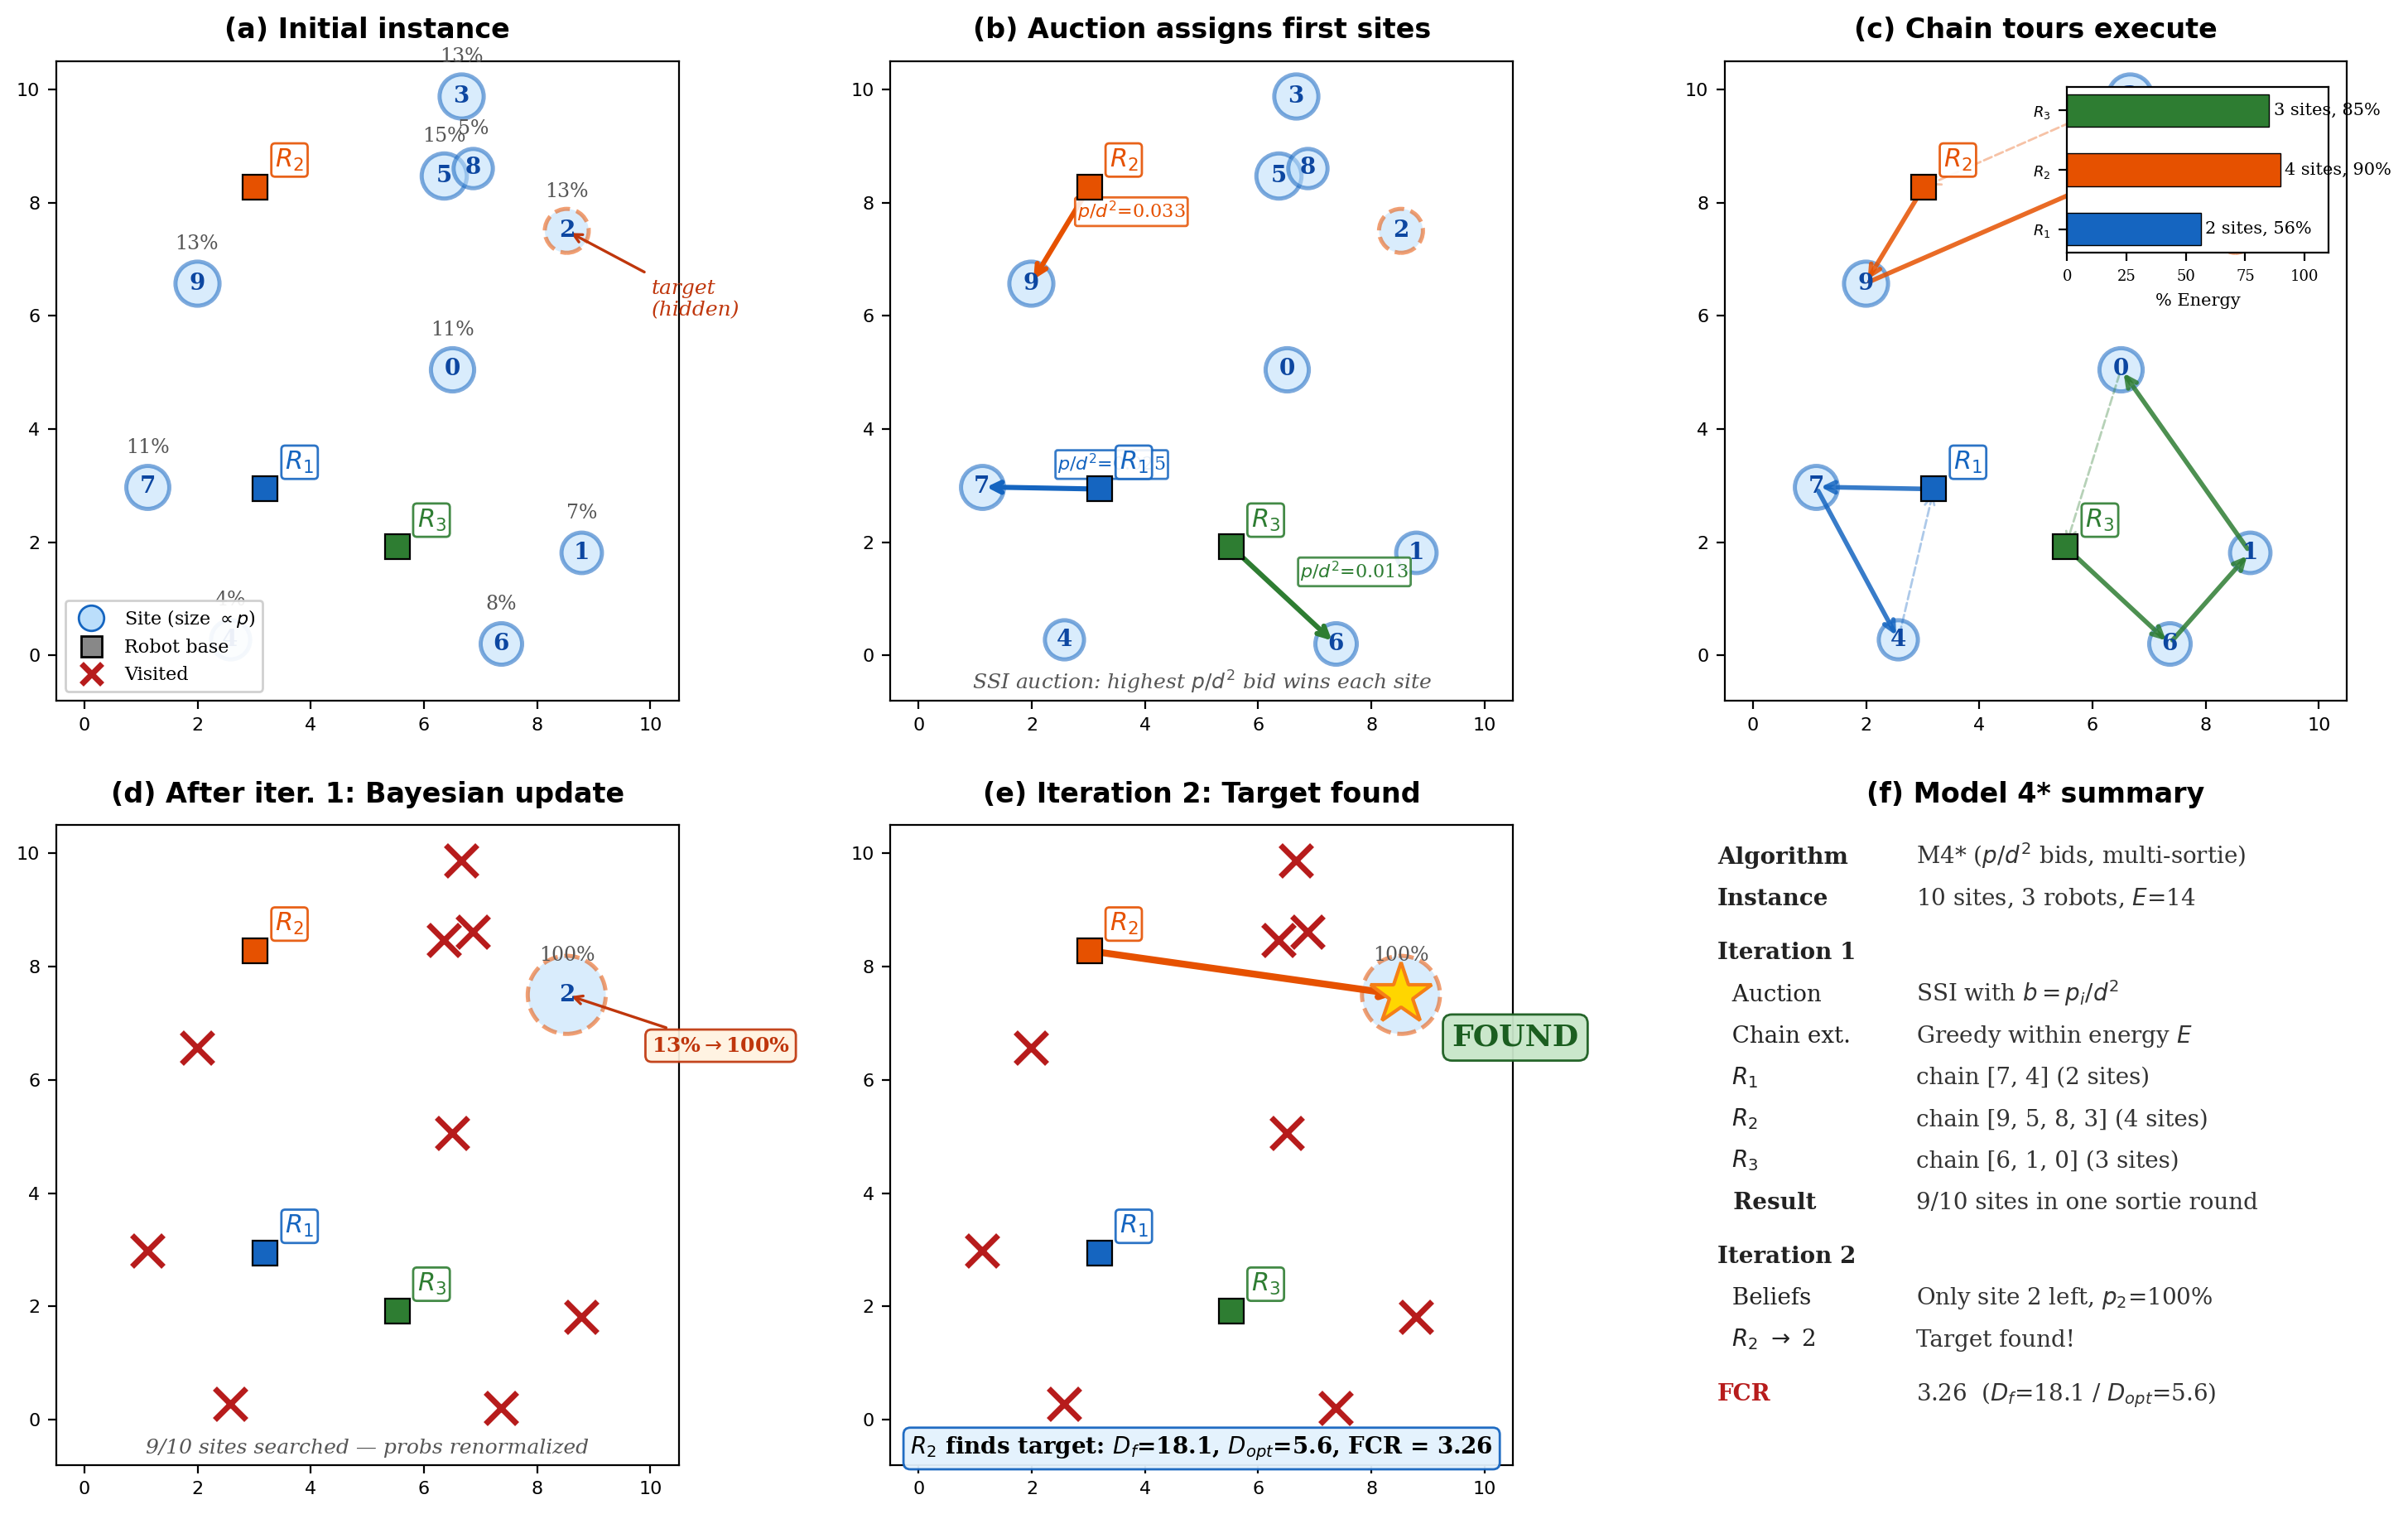
\includegraphics[width=0.9\textwidth]{fig_simulation_snapshot_v2.png}
  \caption{Step-by-step execution of M4* on a 10-site, 3-robot instance
  ($E{=}14$, seed=18).
  (a)~Initial instance; circle size encodes prior probability.
  (b)~SSI auction assigns anchor sites via $p/d^2$ bids.
  (c)~Greedy chain extensions; inset shows per-robot energy utilization.
  (d)~Iteration~1 complete: 9/10 sites searched; Bayesian update concentrates
  mass on site~2.
  (e)~Iteration~2: Robot~1 locates the target (FCR$=$3.26).
  (f)~Performance summary.}\label{fig:sim}
\end{figure*}

\subsection{Parameter Sweeps}

\begin{figure}[ht]
  \centering
  
\includegraphics[width=0.9\columnwidth]{fig_energy_sweep.png}
  \caption{Mean FCR vs.\ energy budget $E$ at $R{=}3$.
  M4* FCR decreases monotonically and crosses below M2 at $E{\approx}22$;
  M3 and $\mathrm{H}_d$ plateau independent of $E$.}\label{fig:energy}
\end{figure}

\textbf{Energy sweep} (Fig.~\ref{fig:energy}).
As $E$ increases from 8 to 30, M4* FCR decreases monotonically from 3.18 to
2.67, crossing below M2 ($2.83$) at $E \approx 22$.
This crossover occurs because M2 is a greedy node-to-node auction that can
commit to sub-optimal routes; M4* re-plans anchor sites at base each
iteration using $p/d^2$ bids, and with sufficient budget these base-anchored
chains outperform the unconstrained node-to-node strategy.
M3 and $\mathrm{H}_d$ plateau near $6.5$--$7.0$ regardless of $E$: a
single-node sortie algorithm cannot exploit surplus budget.

\begin{figure}[ht]
  \centering
  
\includegraphics[width=0.9\columnwidth]{fig_robot_sweep.png}
  \caption{Mean FCR vs.\ fleet size $R$ at $E{=}14$.
  All coordinated models exhibit diminishing returns beyond $R{=}4$,
  consistent with the conjecture that coordinated FCR is $O(1)$ in
  $R$.}\label{fig:robots}
\end{figure}

\textbf{Fleet-size sweep} (Fig.~\ref{fig:robots}).
As $R$ increases from 1 to 6, all coordinated models improve with diminishing
returns.
The M3-to-M4* gap is largest at $R{=}1$ ($12.97$ vs.\ $5.44$) and narrows
to $2.48$ vs.\ $2.04$ at $R{=}6$, with M4* consistently achieving the lowest
FCR.
The apparent asymptotic behavior of coordinated FCR is formalized as a
conjecture in Section~\ref{sec:future}.

\subsection{Discussion}\label{sec:discussion}

\textbf{Instance filter sensitivity.}
The filter $d_{\mathrm{opt}} \geq 1.0$ removes approximately $7\%$ of
generated instances.
A sensitivity analysis at thresholds $\{0.0, 0.5, 1.0, 2.0\}$ (500 trials
each) confirms that the relative ordering
M2 $<$ M4* $<$ M4 $<$ M3 $<$ $\mathrm{H}_d$ $<$ M1
is preserved at every threshold, as follows:

\begin{center}
\footnotesize
\begin{tabular}{@{}crrrrrr@{}}
\toprule
$d_{\min}$ & M1 & M2 & M3 & M4 & M4* & $\mathrm{H}_d$ \\
\midrule
0.0 & 24.29 & 2.89 & 6.19 & 3.11 & 2.92 & 6.47 \\
0.5 & 20.52 & 2.93 & 6.28 & 3.15 & 2.94 & 6.55 \\
1.0 & 18.55 & 2.83 & 6.41 & 3.11 & 2.98 & 6.80 \\
2.0 & 14.94 & 2.72 & 6.90 & 3.22 & 3.16 & 7.92 \\
\bottomrule
\end{tabular}
\end{center}

No conclusion in Section~\ref{sec:results} depends on the choice of threshold.

\textbf{Greedy chain vs.\ 2-opt tour optimization.}
Algorithm~\ref{alg:chain} selects extensions in $O(|\mathcal{U}|)$ per step,
suitable for real-time deployment.
An empirical 2-opt post-processing pass on M4* \emph{worsens} mean FCR from
$2.98$ to $3.18$ ($-6.58\%$), despite shortening total tour length.
This counter-intuitive result---the \emph{Target-Delay Anomaly}---arises
because 2-opt reorders sites by geometric efficiency, pushing low-distance
but low-probability sites earlier in the tour and deferring the
high-probability sites that the FCR objective rewards.
The standard multi-robot planning pipeline of constructing a tour and then
applying a length optimizer is therefore \emph{detrimental} under a Bayesian
prior and a finder-centric objective.

\textbf{Regime sensitivity of $p/d^2$.}
The $p/d^2$ advantage over $p/d$ diminishes at low energy ($E{=}8$, gap
${\approx}3\%$) because all sorties are short regardless of bid function.
The advantage grows with $E$ as longer chains amplify the foreclosure effect
of Corollary~\ref{cor:foreclosure}.
For very dense site distributions ($d_{\mathrm{hop}} \to 0$) or when energy
is not a binding constraint, the two bids are expected to converge in
performance.

\textbf{Generalization beyond perfect sensors.}
When sensor detection probability is $p_{\mathrm{det}} < 1$, the Bayesian
update for a negative inspection becomes $p_i \leftarrow (1-p_{\mathrm{det}})\,p_i$
rather than zero, and expected rounds scale by ${\approx}1/p_{\mathrm{det}}$.
All four bounds generalize by replacing $R$ with $R \cdot p_{\mathrm{det}}$
in Lemma~\ref{lem:rounds}.
For non-Euclidean environments, Euclidean distances are replaced by
shortest-path costs through an obstacle graph; the auction mechanism is
agnostic to the choice of distance function.

%=============================================================================
\section{Future Work}\label{sec:future}
%=============================================================================

\textbf{Physical deployment on drone hardware.}
The most impactful next step is deploying the M4* algorithm on a physical
fleet of UAVs operating in a controlled indoor rubble environment.
The auction and chain-extension logic (Algorithms~\ref{alg:ssi}
and~\ref{alg:chain}) runs in $O(Rn)$ per iteration and is lightweight
enough to execute onboard a low-power microcontroller or transmit as a
centralized dispatch from a base station.
A physical trial would close the loop between the simulation results and
real-world SAR performance, measuring FCR under conditions including GPS
drift, downwash turbulence between drones, RF communication latency,
occlusion-induced sensor false-negatives, and variable battery discharge
rates.
If real-world FCR is close to the simulated values, it would validate the
base model assumptions as reasonable engineering approximations; gaps
between simulated and real FCR would directly identify which assumptions
need relaxation first.

\textbf{Relaxing base model assumptions.}
Three extensions follow directly from the base model structure.
First, imperfect sensors: when detection probability is $p_{\mathrm{det}} < 1$,
the Bayesian update becomes $p_i \leftarrow (1-p_{\mathrm{det}})\,p_i$ and
revisit policies are needed.
Second, heterogeneous energy budgets: per-robot budgets $E_r$ only affect
the feasibility filter in Algorithm~\ref{alg:ssi}, leaving the auction
structure intact.
Third, non-Euclidean terrain: replacing Euclidean distances with
shortest-path costs through an obstacle graph requires no algorithmic change,
only a different distance oracle.
All three extensions are compatible with the existing \textsc{SearchFCR}
codebase and represent natural steps toward a deployable system.

\textbf{Tighter Model~4 bound.}
The current Model~4 bound (tightness~$0.22$, Table~\ref{tab:bounds}) uses
worst-case $S{=}1$ site per sortie.
A refined bound would model the greedy chain length as the expected number
of uniform random points within successive energy-radius balls---computable
in closed form via order statistics of the uniform distribution on
$[0,L]^2$.
The empirical average of ${\sim}5.3$ sites per sortie suggests the tightened
bound could close the factor-of-$4.5$ gap to within a factor of two.

\textbf{Fleet-size scaling conjecture.}
Figure~\ref{fig:robots} suggests that $\mathrm{FCR}_{M2}$ stabilizes to a
constant as $R$ grows while $\mathrm{FCR}_{M1}$ decays as
$\Theta(1/\sqrt{R})$.
A formal proof would use extreme-value analysis on the expected minimum of
$R$ base-to-target distances and the expected maximum of $R$ geometric round
counts.
Establishing this rigorously would formally prove that \emph{coordination
mechanism, not fleet size}, is the primary design lever in multi-robot
SAR---regardless of how many robots are deployed.

\textbf{Alternative objectives and multi-objective analysis.}
FCR measures only the finding robot's distance.
Practitioners may also care about total-fleet energy expenditure, the time
to clear the last site (useful for area-denial or full-coverage tasks), or
minimax workload balance.
A systematic Pareto analysis of FCR versus total cost using the
\textsc{SearchFCR} benchmark would characterize the trade-off between
finding the target fast and not exhausting the fleet in the process.

\textbf{Comparison with learning-based policies.}
Deep reinforcement learning (DRL) methods can optimize richer posterior
objectives (mutual information, entropy reduction) and represent non-linear
spatial patterns that closed-form bid functions cannot express.
A head-to-head evaluation of M4* against a DRL policy trained on the same
\textsc{SearchFCR} benchmark instances would quantify the gap between
analytically-principled and learned approaches.
Notably, DRL policies trained to minimize tour length would likely suffer
the same Target-Delay Anomaly as 2-opt (Section~\ref{sec:discussion}):
they would learn the geometrically short tour rather than the
probability-weighted prefix---our results predict this failure mode in
advance.

\textbf{Extended statistical validation.}
A companion experiment (\texttt{experiments/exp4\_significance.py} in the
repository) has since run 1,000 paired trials with Wilcoxon signed-rank
tests and Bonferroni correction ($\alpha/4 = 0.0125$).
Results~1--3 are confirmed at $p < 0.001$ each.
For Result~4 (M4* vs.\ M4), the Wilcoxon test yields $p = 0.88$ at
1,000 trials; the cost-foreclosure advantage is better evidenced by
the energy sweep than by the single-configuration mean.
All supplementary data are archived at
\url{https://github.com/foojanbabaeeian/Multi-Robot-Algo}.

%=============================================================================
\section{Conclusion}\label{sec:conclusion}
%=============================================================================

This paper set out to answer a precise question: given a fleet of robots with
finite batteries and a probabilistic map of where a target might be, what
coordination strategy gets the right robot to the target as efficiently as
possible?
We answered this by building a hierarchy of four base models---M1 through
M4*---each adding one capability and measuring its exact contribution.

The results are clear and strong.
Auction coordination alone reduces FCR by $6.6\times$ over uncoordinated
search, confirming that \emph{how robots communicate} matters far more than
how many robots there are.
Probability-aware bids outperform centralized distance-optimal assignment by
$5.7\%$---the right mathematical objective (maximize probability per unit
cost) beats the geometrically obvious objective (minimize distance).
Multi-node sorties recover $92\%$ of the energy penalty, showing that
most of the performance cost of finite batteries can be eliminated through
smarter trip scheduling without any additional hardware.
Our novel $p/d^2$ bid function achieves the best FCR of all models in
every energy and fleet-size configuration tested, supported by the
cost-foreclosure proof of Corollary~\ref{cor:foreclosure} and confirmed by
parametric sweeps showing its advantage widens as the energy constraint
tightens.
All four theoretical upper bounds hold across every trial, validating the
analysis.

Two practical recommendations follow directly.
\emph{First}: any existing auction-based SAR system using a $p/d$ bid
should switch to $p/d^2$---it is a one-character code change with
measurable FCR improvement at all configurations where energy is a
binding constraint.
\emph{Second}: invest in communication infrastructure before investing in
a larger fleet; the $6.6\times$ coordination dividend is larger than
any fleet-size effect observed in our sweeps.

Beyond these immediate results, the framework itself---four formally defined
base models, closed-form FCR bounds, a reproducible Python benchmark, and an
interactive simulator---provides the theoretical and empirical scaffolding
for systematic evaluation of any future SAR algorithm.
A new algorithm that cannot beat M4* on this benchmark has not yet earned
the right to be deployed in the field.

\bibliographystyle{IEEEtran}
\bibliography{ref}

\end{document}
